\subsection{ceres-solver}

\begin{frame}
   \frametitle{Ceres-solver}
    
    Доступные решатели:

    \begin{itemize}
      \item Spteepest descent 
      \item Nonlinear conjugate gradients
      \item BFGS
      \item L-BFGS 
    
    \end{itemize} 
    
    Поддержка Wolfe и Armijo conditions.

\end{frame}


\defverbatim[colored]\lstI{
\begin{lstlisting}[language=C++,basicstyle=\ttfamily\tiny,keywordstyle=\color{red}]
class Rosenbrock : public ceres::FirstOrderFunction {
 public:
  virtual ~Rosenbrock() {}
  virtual bool Evaluate(const double* parameters,
                        double* cost,
                        double* gradient) const {
    const double x = parameters[0];
    const double y = parameters[1];
    cost[0] = (1.0 - x) * (1.0 - x) + 100.0 * (y - x * x) * (y - x * x);
    if (gradient != NULL) {
      gradient[0] = -2.0 * (1.0 - x) - 200.0 * (y - x * x) * 2.0 * x;
      gradient[1] = 200.0 * (y - x * x);
    }
    return true;
  }
  virtual int NumParameters() const { return 2; }
};
\end{lstlisting}
}

\subsection{Rosenbrock function}
\begin{frame}
  \frametitle{Rosenbrock function}
  \begin{equation*}
    (1-x)^2 + 100(y-x^2)^2
  \end{equation*}

  \begin{equation*}
    min : (1, 1)
  \end{equation*}

  \begin{figure}
    \centering
    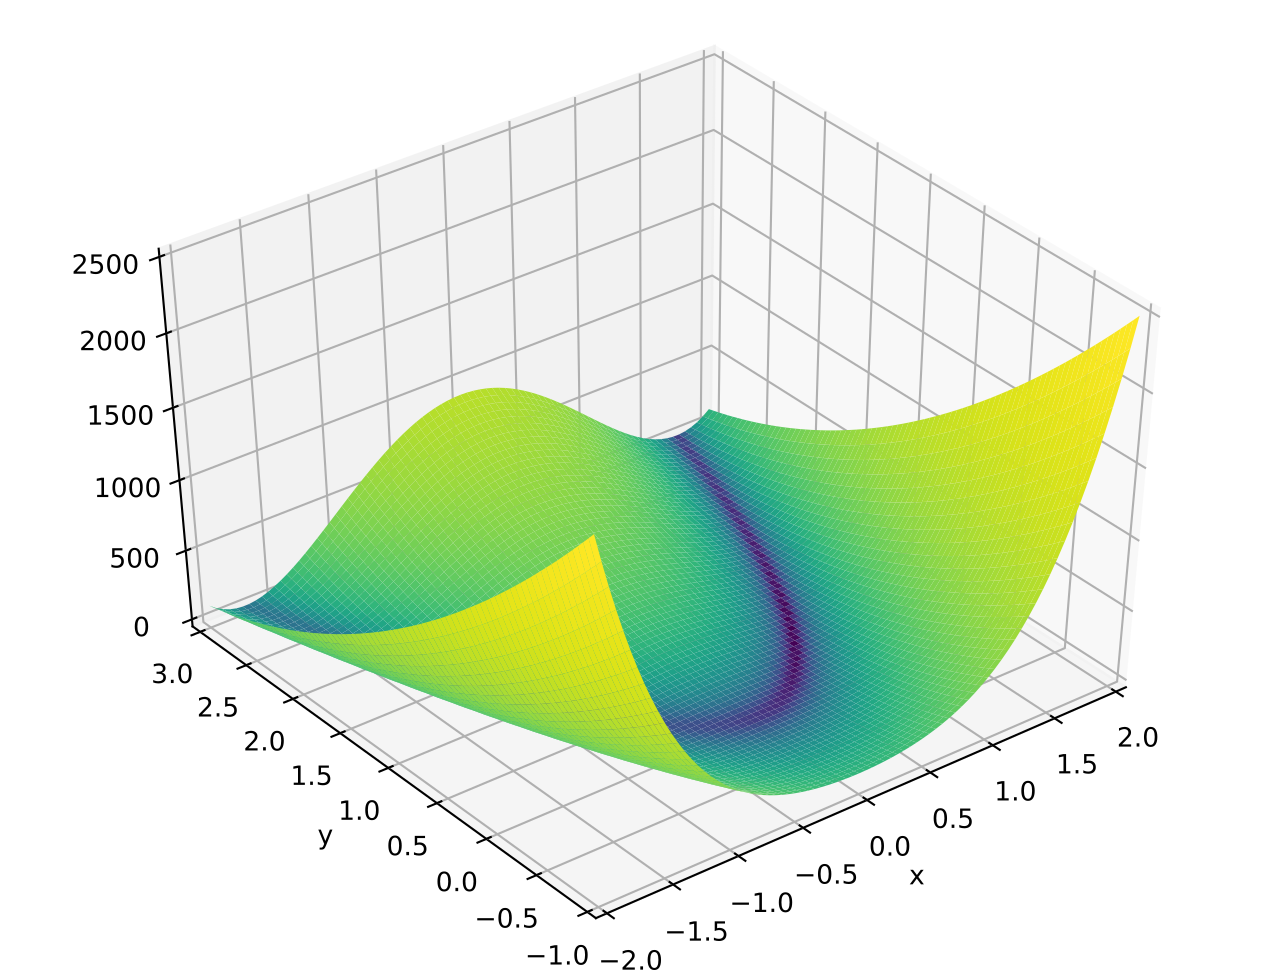
\includegraphics[width=6cm]{figures/rosenbrock.png}
  \end{figure}

\end{frame}

\subsection{ceres-solver code}
\begin{frame}[fragile]
  \frametitle{Rosenbrock function}
\lstI    
\end{frame}


\defverbatim[colored]\lstR{
\begin{lstlisting}[basicstyle=\ttfamily\tiny]
   0: f: 2.420000e+01 d: 0.00e+00 g: 2.16e+02 h: 0.00e+00 s: 0.00e+00 e:  0 it: 1.00e-05 tt: 1.00e-05
   1: f: 4.280493e+00 d: 1.99e+01 g: 1.52e+01 h: 2.01e-01 s: 8.62e-04 e:  2 it: 6.32e-05 tt: 1.29e-04
   2: f: 3.571154e+00 d: 7.09e-01 g: 1.35e+01 h: 3.78e-01 s: 1.34e-01 e:  3 it: 2.19e-05 tt: 1.68e-04
  32: f: 1.003030e-12 d: 1.90e-09 g: 3.50e-05 h: 3.52e-05 s: 1.00e+00 e:  1 it: 3.81e-06 tt: 5.24e-04
  33: f: 4.835994e-17 d: 1.00e-12 g: 1.05e-07 h: 1.13e-06 s: 1.00e+00 e:  1 it: 4.05e-06 tt: 5.38e-04
  34: f: 1.885250e-22 d: 4.84e-17 g: 2.69e-10 h: 1.45e-08 s: 1.00e+00 e:  1 it: 4.05e-06 tt: 5.48e-04

Parameters                                  2
Line search direction              LBFGS (20)
Line search type                  CUBIC WOLFE

Cost:
Initial                          2.420000e+01
Final                            1.955192e-27
Change                           2.420000e+01

Minimizer iterations                       36

Time (in seconds):
  Cost evaluation                    0.000000 (0)
  Gradient & cost evaluation         0.000010 (44)
  Polynomial minimization            0.000071
Total                                0.000589

Termination:    CONVERGENCE (Parameter tolerance reached. Relative step norm: 1.890726e-11 <= 1.000000e-08.)

Initial x: -1.2 y: 1
Final   x: 1 y: 1
\end{lstlisting}
}

\begin{frame}[fragile]
  \frametitle{Пример вывода}
  \lstR
\end{frame}

